%============================================================================%
%
%	DOCUMENT DEFINITION
%
%============================================================================%

\documentclass[10pt,A4]{article}	


%============================================================================%
%
%	ENCODING
%
%============================================================================%

\usepackage[utf8]{inputenc}		

%============================================================================%
%
%	LOGIC
%
%============================================================================%

\usepackage{xifthen}

%============================================================================%
%
%	FONT
%
%============================================================================%

% some tex-live fonts - choose your own

%\usepackage[defaultsans]{droidsans}
%\usepackage[default]{comfortaa}
%\usepackage{cmbright}
%\usepackage[default]{raleway}
%\usepackage{fetamont}
\usepackage[default]{gillius}
%\usepackage[light,math]{iwona}
%\usepackage[thin]{roboto}
\usepackage{amssymb}

% set font default
\renewcommand*\familydefault{\sfdefault} 	
\usepackage[T1]{fontenc}

% more font size definitions
\usepackage{moresize}		

\usepackage{fontawesome}

%----------------------------------------------------------------------------------------
%	PAGE LAYOUT  DEFINITIONS
%----------------------------------------------------------------------------------------

%debug page outer frames
%\usepackage{showframe}			


%define page styles using geometry
\usepackage[a4paper]{geometry}		

% for example, change the margins to 2 inches all round
\geometry{top=1cm, bottom=-.6cm, left=0.4cm, right=1cm} 	


%less space between header and content
\setlength{\headheight}{-5pt}		

%indentation is zero
\setlength{\parindent}{0mm}

%----------------------------------------------------------------------------------------
%	TABLE /ARRAY DEFINITIONS
%---------------------------------------------------------------------------------------- 

%for layouting tables
\usepackage{multicol}			
\usepackage{multirow}

%extended aligning of tabular cells
\usepackage{array}

\newcolumntype{x}[1]{%
>{\raggedleft\hspace{0pt}}p{#1}}%


%----------------------------------------------------------------------------------------
%	GRAPHICS DEFINITIONS
%---------------------------------------------------------------------------------------- 

%for header image
\usepackage{graphicx}

%for floating figures
\usepackage{wrapfig}
\usepackage{float}
%\floatstyle{boxed} 
%\restylefloat{figure}

%for drawing graphics		
\usepackage{tikz}				
\usetikzlibrary{shapes, backgrounds,mindmap, trees}


%----------------------------------------------------------------------------------------
%	Color DEFINITIONS
%---------------------------------------------------------------------------------------- 
\usepackage{transparent}
\usepackage{color}

%accent color
\definecolor{complcol}{RGB}{250,150,10}

%dark background color
\definecolor{bgcol}{RGB}{110,110,110}

%light background / accent color
\definecolor{softcol}{RGB}{225,225,225}

\definecolor{sectcol}{RGB}{0,120,150}


%Package for links, must be the last package used
\usepackage[hidelinks]{hyperref}

%============================================================================%
%
%
%	DEFINITIONS
%
%
%============================================================================%

% returns minipage width minus two times \fboxsep
% to keep padding included in width calculations
\newcommand{\mpwidth}{\linewidth-\fboxsep-\fboxsep}
	

%----------------------------------------------------------------------------------------
% 	ARROW GRAPHICS in Tikz
%----------------------------------------------------------------------------------------

% a six pointed arrow poiting to the left
\newcommand{\tzlarrow}{(0,0) -- (0.2,0) -- (0.3,0.2) -- (0.2,0.4) -- (0,0.4) -- (0.1,0.2) -- cycle;}	

% include the left arrow into a tikz picture
% param1: fill color
%
\newcommand{\larrow}[1]
{\begin{tikzpicture}[scale=0.58]
	 \filldraw[fill=#1!100,draw=#1!100!black]  \tzlarrow
 \end{tikzpicture}
}

% a six pointed arrow poiting to the right
\newcommand{\tzrarrow}{ (0,0.2) -- (0.1,0) -- (0.3,0) -- (0.2,0.2) -- (0.3,0.4) -- (0.1,0.4) -- cycle;}

% include the right arrow into a tikz picture
% param1: fill color
%
\newcommand{\rarrow}
{
\begin{tikzpicture}[scale=0.7]
	\filldraw[fill=sectcol!100,draw=sectcol!100!black] \tzrarrow
 \end{tikzpicture}
}

%----------------------------------------------------------------------------------------
%	custom sections
%----------------------------------------------------------------------------------------

% create a coloured box with arrow and title as cv section headline
% param 1: section title
%
\newcommand{\cvsection}[1]
{
\colorbox{sectcol}{\mystrut \makebox[1\mpwidth][l]{
\vspace{2pt}\hspace{2pt}\textbf{\textcolor{white}{\normalsize\uppercase{#1}}}\hspace{4pt}
}}\\
}

% create a coloured arrow with title as cv meta section section
% param 1: meta section title
%
\newenvironment{metasection}[1] {
	\vspace{6pt}
	\begin{center}
		\textcolor{white}{\large{\uppercase{#1}}}\\
	\normalsize
	\parbox{0.7\mpwidth}{\textcolor{white}	\hrule}
}{\end{center}}

%----------------------------------------------------------------------------------------
%	 CV EVENT
%----------------------------------------------------------------------------------------

\newcommand{\cveventNow}[9]
{
	\vspace{8pt}
	\begin{tabular*}{1\mpwidth}{p{0.55\mpwidth}  x{0.42\mpwidth}}
		\textcolor{black}{\textbf{#2}} & \textcolor{complcol}{#3},
		\textcolor{bgcol}{#1} 
		
		
	\end{tabular*}
	\vspace{-12pt}
	\textcolor{softcol}{\hrule}
	\vspace{6pt}
	\begin{tabular*}{0.5\mpwidth}{p{\mpwidth}}
		\larrow{softcol}  #4\\[4pt]
		\larrow{softcol}  #5\\[4pt]
		\larrow{softcol}  #6\\[4pt]
		\larrow{softcol}  #7\\[4pt]
		\larrow{softcol}  #8\\[4pt]
		\larrow{softcol}  #9\\[4pt]
	\end{tabular*}
	
}

\newcommand{\cveventMbc}[9]
{
	\vspace{8pt}
	\begin{tabular*}{1\mpwidth}{p{0.55\mpwidth}  x{0.42\mpwidth}}
		\textcolor{black}{\textbf{#2}} & \textcolor{complcol}{#3},
		\textcolor{bgcol}{#1} 
		
		
	\end{tabular*}
	\vspace{-12pt}
	\textcolor{softcol}{\hrule}
	\vspace{6pt}
	\begin{tabular*}{0.5\mpwidth}{p{\mpwidth}}
		\larrow{softcol}  #4\\[4pt]
		\larrow{softcol}  #5\\[4pt]
		\larrow{softcol}  #6\\[4pt]
		\larrow{softcol}  #7\\[4pt]
		\larrow{softcol}  #8\\[4pt]
		\larrow{softcol}  #9\\[4pt]
	\end{tabular*}
	
}

\newcommand{\cveventExxeta}[9]
{
	\vspace{8pt}
	\begin{tabular*}{1\mpwidth}{p{0.55\mpwidth}  x{0.42\mpwidth}}
		\textcolor{black}{\textbf{#2}} & \textcolor{complcol}{#3},
		\textcolor{bgcol}{#1} 
		
		
	\end{tabular*}
	\vspace{-12pt}
	\textcolor{softcol}{\hrule}
	\vspace{6pt}
	\begin{tabular*}{0.5\mpwidth}{p{\mpwidth}}
		\larrow{softcol}  #4\\[4pt]
		\larrow{softcol}  #5\\[4pt]
		\larrow{softcol}  #6\\[4pt]
		\larrow{softcol}  #7\\[4pt]
		\larrow{softcol}  #8\\[4pt]
		\larrow{softcol}  #9\\[4pt]
	\end{tabular*}
	
}

\newcommand{\cveventMaster}[7]
{
	\vspace{8pt}
	\begin{tabular*}{1\mpwidth}{p{0.55\mpwidth}  x{0.42\mpwidth}}
		\textcolor{black}{\textbf{#2}} & \textcolor{complcol}{#3},
		\textcolor{bgcol}{#1} 
		
		
	\end{tabular*}
	\vspace{-12pt}
	\textcolor{softcol}{\hrule}
	\vspace{6pt}
	\begin{tabular*}{0.5\mpwidth}{p{\mpwidth}}
		\larrow{softcol}  #4\\[4pt]
		\larrow{softcol}  #5\\[4pt]
		\larrow{softcol}  #6\\[4pt]
		\larrow{softcol}  #7\\[4pt]
	\end{tabular*}
	
}

\newcommand{\cveventGlasgow}[6]
{
	\vspace{8pt}
	\begin{tabular*}{1\mpwidth}{p{0.55\mpwidth}  x{0.42\mpwidth}}
		\textcolor{black}{\textbf{#2}} & \textcolor{complcol}{#3},
		\textcolor{bgcol}{#1} 
		
		
	\end{tabular*}
	\vspace{-12pt}
	\textcolor{softcol}{\hrule}
	\vspace{6pt}
	\begin{tabular*}{0.5\mpwidth}{p{\mpwidth}}
		\larrow{softcol}  #4\\[4pt]
		\larrow{softcol}  #5\\[4pt]
		\larrow{softcol}  #6\\[4pt]
	\end{tabular*}
	
}

% creates a stretched box as 
\newcommand{\cveventmeta}[2]
{
	\mbox{\mystrut \hspace{87pt}\textit{#1}}\\
	#2
}

%----------------------------------------------------------------------------------------
% CUSTOM STRUT FOR EMPTY BOXES
%----------------------------------------- -----------------------------------------------
\newcommand{\mystrut}{\rule[-.3\baselineskip]{0pt}{\baselineskip}}

%----------------------------------------------------------------------------------------
% CUSTOM LOREM IPSUM
%----------------------------------------------------------------------------------------
\newcommand{\lorem}
{Lorem ipsum dolor sit amet, consectetur adipiscing elit. Donec a diam lectus.}

\newcommand{\vcenteredinclude}[1]{\begingroup
\setbox0=\hbox{\includegraphics{#1}}%
\parbox{\wd0}{\box0}\endgroup}

\newcommand*{\vcenteredhbox}[1]{\begingroup
\setbox0=\hbox{#1}\parbox{\wd0}{\box0}\endgroup}

%----------------------------------------------------------------------------------------
%	ICON-SET EMBEDDING
%---------------------------------------------------------------------------------------- 

\newcommand{\icon}[3]{\makebox(#2, #2){\textcolor{#3}{\csname fa#1\endcsname}}}	
\newcommand{\icontext}[4]{
	\vcenteredhbox{\icon{#1}{#2}{#4}} \vcenteredhbox{\textcolor{#4}{#3}}
}
\newcommand{\iconhref}[5]{
    \vcenteredhbox{\icon{#1}{#2}{#5}} \href{#4}{\textcolor{#5}{#3}}
}

\newcommand{\iconemail}[5]{ 						%icon with email link
    \vcenteredhbox{\icon{#1}{#2}{#5}} \href{mailto:#4}{\textcolor{#5}{#3}}
}



%============================================================================%
%
%
%
%	DOCUMENT CONTENT
%
%
%
%============================================================================%
\begin{document}
\fcolorbox{white}{white}{\begin{minipage}[c][0.95\textheight][t]{0.69\linewidth}


%---------------------------------------------------------------------------------------
%	TITLE HEADLINE
%----------------------------------------------------------------------------------------
\vspace{-3pt}

% use this for single words, e.g. CV or RESUME etc.
\colorbox{bgcol}{\makebox[\mpwidth][c]{\HUGE{\textcolor{white}{Mikhail Smolin}} \textcolor{sectcol}{\rule[-.2mm]{1mm}{1cm}} \parbox[b]{5.5cm}{
\Large{\textcolor{white}{{e-Discovery Expert}}}\\
\normalsize{\textcolor{white}{{Daimler AG, Stuttgart, Germany}}}

}}}

\vspace{12pt}

%============================================================================%
%
%	CV SECTIONS AND EVENTS (MAIN CONTENT)
%
%============================================================================%

%---------------------------------------------------------------------------------------
%	SUMMARY
%----------------------------------------------------------------------------------------
\cvsection{Summary}

Software expert and computer science (MSc) graduate pushing several years of international IT project experience. Having a strong background in the automotive industry as well as leading distributed engineering teams, I'm highly committed to end-to-end project development; from creating requirements and interfaces to the coordination of agile software development and validation tasks. I have an analytical, result-driven mindset and I am very passionate about cyber security, electronic discovery, web technologies and data protection. Not only I am a dedicated team player who is committed to achieving outstanding work results but also I'm fascinated by research and innovation where I have a great interest in expanding my knowledge as well as experiencing new professional and personal challenges in an international context.

\vspace{12pt}

%---------------------------------------------------------------------------------------
%	EXPERIENCE
%----------------------------------------------------------------------------------------
\cvsection{Experience}

\cveventNow{4/20 - now}{Expert}{Daimler AG}{Responsible for identifying, collecting and processing of electronically stored information.}{In progress...}{In progress...}{In progress...}{In progress...}{In progress...}

\cveventMbc{7/19 - 3/20}{Senior IT Architect}{Mercedes-Benz AG}{Supported driving digital transformation efforts across the broader powertrain landscape.}{Analyzed processes and requirements with international cross-departmental specialists.}{Collaborated with teams across production plants, to help and define the user experience.}{Approved implementations, supported and coordinated engineers and external partners.}{Support of IT at international locations, especially within the scope of piloting new APIs.}{Participated in various work packages of complex cross-plant strategic Daimler IT projects.}

\cveventExxeta{2/17 - 6/19}{Software Engineer and Consultant}{EXXETA AG}{Lead distributed development teams according to Scrum in an agile project setup.}{Full-stack UI/UX Web development for major automotive OEMs and Tier 1 suppliers.}{Interpersonal communication in inter-cultural teams and across multiple time zones.}{Planned and directed all aspects of people activities within the engineering team.}{Managed budget and personnel including tracking and communication to stakeholders.}{Collaborated with external companies to develop long-term strategic partnerships.}

\vspace{12pt}

%============================================================================%
%
%	EUDUCATION
%
%============================================================================%

\cvsection{Education}

\cveventMaster{3/14 - 1/17}{Computer Science, MSc $\varnothing$ 1.3}{Stuttgart Media University}{Master's thesis (1.0): «Anomaly-based intrusion detection for automotive networks»}{I proposed the applicability of detecting cyber attacks on the vehicular CAN bus.}{By means of a self-learning mechanism, a neural network was trained and evaluated.}{Courses: software engineering, data privacy, secure systems, agile project management.}

\cveventGlasgow{9/15 - 2/16}{Computer Science, MSc}{University of Glasgow}{I successfully attended courses in data mining, cyber security and intermediate English.}{Implementation of an Android diagnostics tool from vehicle's sensor data using Java.}{Project: mobile car diagnostics and performance app from vehicular on-board data.}

\end{minipage}}%
\fcolorbox{white}{sectcol}{\begin{minipage}[c][0.95\textheight][t]{0.33\linewidth}

\vspace{18pt}	
\begin{center}
	{
		\setlength{\fboxsep}{0pt}%
		\setlength{\fboxrule}{0pt}%
		\fbox{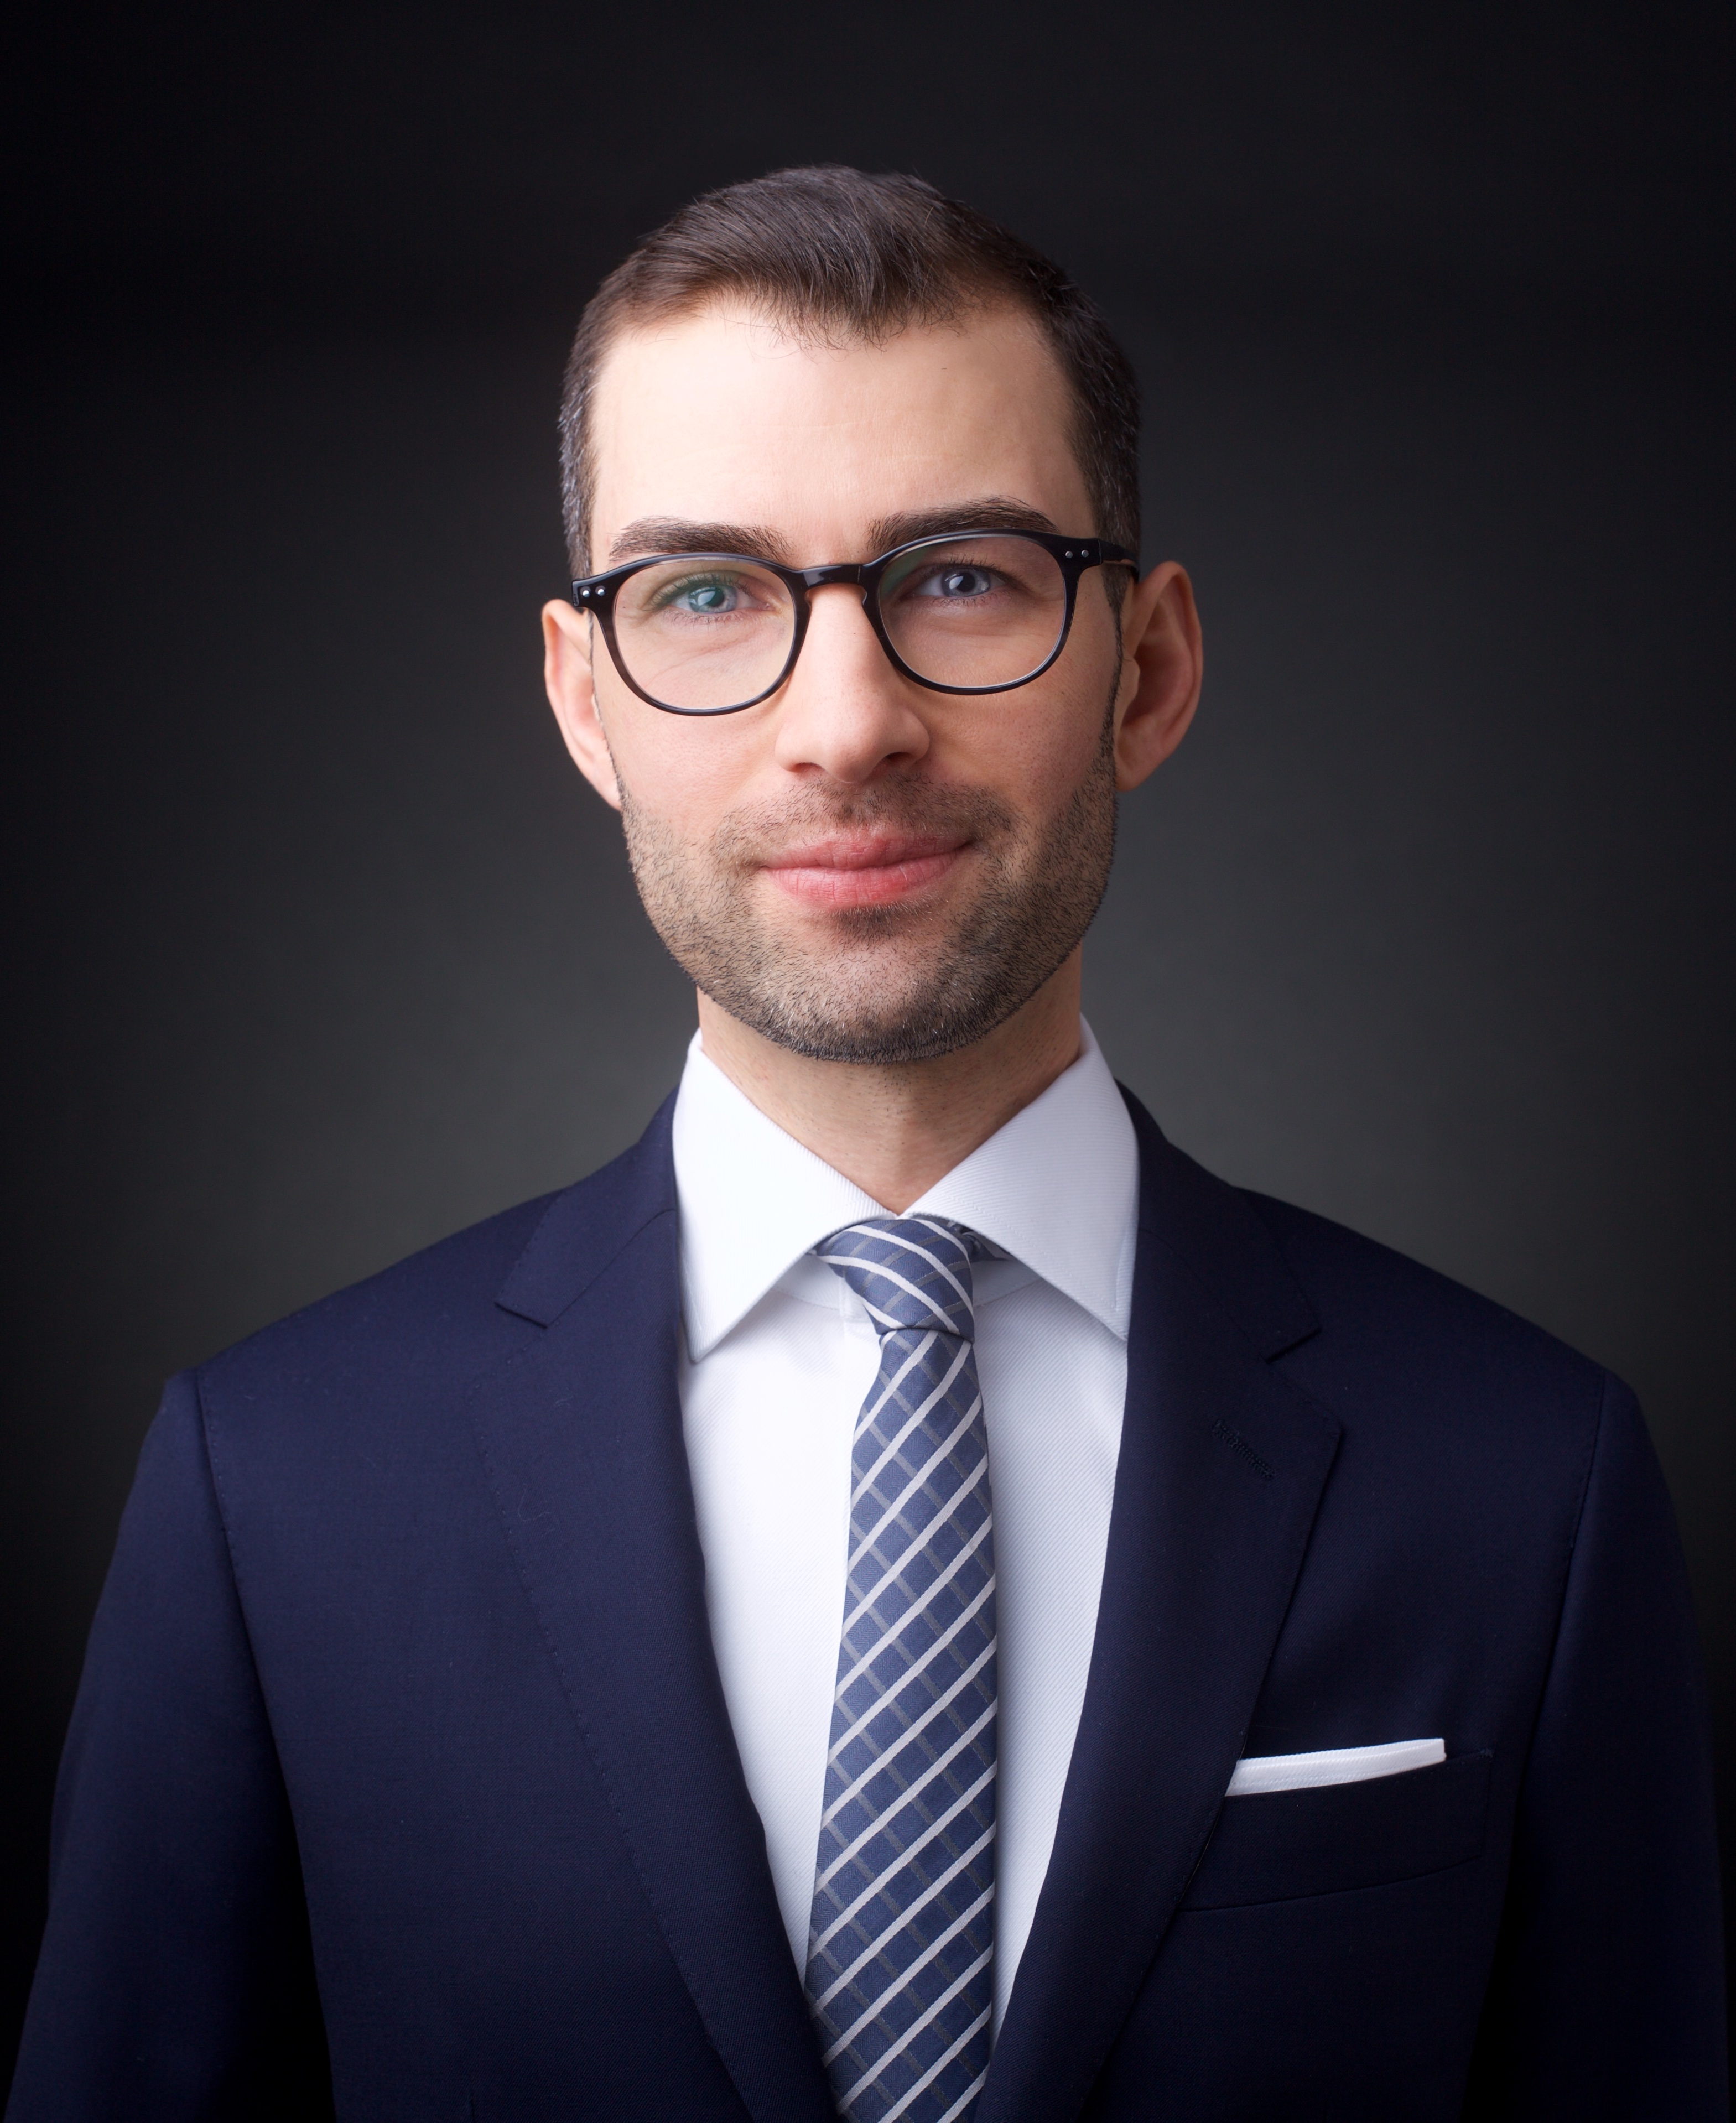
\includegraphics[width=.7\linewidth]{images/me}}
	}
\end{center}

\begin{metasection}{Contact}

	\icontext{MapMarker}{12}{Stuttgart, Germany}{white}\\[6pt]
	\icontext{Phone}{12}{+49 176 30915134}{white}\\[6pt]
	\iconemail{Envelope}{12}{mikhail.smolin@daimler.com}{mikhail.smolin@daimler.com}{white}\\[6pt]
	\iconhref{MousePointer}{12}{smolin.io}{https://smolin.io/}{white}\\[6pt]
	
\end{metasection}
	
%============================================================================%
%
%	META
%
%============================================================================%

\begin{metasection}{Languages}

\icontext{Home}{12}{German (CEFR C2)}{white}\\[6pt]
\icontext{Group}{12}{English (CEFR C1)}{white}\\[6pt]
\icontext{Comments}{12}{Russian (CEFR B2)}{white}\\[6pt]
\icontext{Comment}{12}{Korean (CEFR A1)}{white}\\[6pt]


\end{metasection}

\begin{metasection}{Technologies}

\textcolor{white}{
\icontext{Code}{12}{HTML, JS, JEE, CSS, Python, Matlab}{white}\\[6pt]
\icontext{Fire}{12}{Dojo, React, Django, TensorFlow}{white}\\[6pt]
\icontext{Database}{12}{MySQL, PostgreSQL}{white}\\[6pt]
\icontext{CodeFork}{12}{Git, Travis CI}{white}\\[6pt]
}
\end{metasection}

\begin{metasection}{Tools}

\textcolor{white}{
\icontext{Code}{12}{IntelliJ, VS Code, Atom, PyCharm}{white}\\[6pt] \icontext{CodeFork}{12}{Jira, Confluence, Azure DevOps}{white}\\[6pt]
\icontext{Terminal}{12}{Shell, Docker, Homebrew}{white}\\[6pt]
\icontext{Cube}{12}{Relativity, Nuix, Office}{white}\\[6pt]
}
\end{metasection}

\begin{metasection}{Operating Systems}

\textcolor{white}{\LARGE{\icon{Apple}{24}{white} \icon{Linux}{24}{white}  \icon{Windows}{24}{white}}}

\end{metasection}

\begin{metasection}{Licences}
	
	\textcolor{white}{\LARGE{\icon{Automobile}{24}{white} \icon{Motorcycle}{24}{white}}}
	
\end{metasection}

\vspace{-2pt}

\end{minipage}}

%============================================================================%
%
%	ARTIFICIAL FOOTER
%
%============================================================================%

\null
\vspace*{\fill}
\hspace{-0.25\linewidth}\colorbox{bgcol}{\makebox[1.5\linewidth][c]{\mystrut \small \textcolor{white}{Mikhail Smolin} $\cdot$ \textcolor{white}{2020}}}

\end{document}
